\documentclass[xelatex,aspectratio=169]{beamer}

\hfuzz=10pt
\vfuzz=10pt

% Theme
\usetheme{htw}
\setbeamertemplate{navigation symbols}{}
\setbeamertemplate{theorems}[numbered]
\setbeamercovered{transparent}

%\logo{
\includegraphics[height=0.5cm]{HTWD_color.png}}

% Packages
\usepackage{polyglossia}
\setmainlanguage{german}
\setotherlanguage{english}

\usepackage[bigfiles]{pdfbase}
\ExplSyntaxOn
\NewDocumentCommand\embedvideo{smm}{
\group_begin:
\leavevmode
\tl_if_exist:cTF{file_\file_mdfive_hash:n{#3}}{
  \tl_set_eq:Nc\video{file_\file_mdfive_hash:n{#3}}
}{
  \IfFileExists{#3}{}{\GenericError{}{File~`#3'~not~found}{}{}}
  \pbs_pdfobj:nnn{}{fstream}{{}{#3}}
  \pbs_pdfobj:nnn{}{dict}{
    /Type/Filespec/F~(#3)/UF~(#3)
    /EF~<</F~\pbs_pdflastobj:>>
  }
  \tl_set:Nx\video{\pbs_pdflastobj:}
  \tl_gset_eq:cN{file_\file_mdfive_hash:n{#3}}\video
}
%
\pbs_pdfobj:nnn{}{dict}{
  /Type/RichMediaInstance/Subtype/Video
  /Asset~\video
  /Params~<</FlashVars (
  source=#3&
  skin=SkinOverAllNoFullNoCaption.swf&
  skinAutoHide=true&
  skinBackgroundColor=0x5F5F5F&
  skinBackgroundAlpha=0.75
  )>>
}
%
\pbs_pdfobj:nnn{}{dict}{
/Type/RichMediaConfiguration/Subtype/Video
/Instances~[\pbs_pdflastobj:]
}
%
\pbs_pdfobj:nnn{}{dict}{
/Type/RichMediaContent
/Assets~<<
/Names~[(#3)~\video]
>>
/Configurations~[\pbs_pdflastobj:]
}
\tl_set:Nx\rmcontent{\pbs_pdflastobj:}
%
\pbs_pdfobj:nnn{}{dict}{
  /Activation~<<
  /Condition/\IfBooleanTF{#1}{PV}{XA}
  /Presentation~<</Style/Embedded>>
  >>
  /Deactivation~<</Condition/PI>>
}
%
\hbox_set:Nn\l_tmpa_box{#2}
\tl_set:Nx\l_box_wd_tl{\dim_use:N\box_wd:N\l_tmpa_box}
\tl_set:Nx\l_box_ht_tl{\dim_use:N\box_ht:N\l_tmpa_box}
\tl_set:Nx\l_box_dp_tl{\dim_use:N\box_dp:N\l_tmpa_box}
\pbs_pdfxform:nnnnn{1}{1}{}{}{\l_tmpa_box}
%
\pbs_pdfannot:nnnn{\l_box_wd_tl}{\l_box_ht_tl}{\l_box_dp_tl}{
  /Subtype/RichMedia
  /BS~<</W~0/S/S>>
  /Contents~(embedded~video~file:#3)
  /NM~(rma:#3)
  /AP~<</N~\pbs_pdflastxform:>>
  /RichMediaSettings~\pbs_pdflastobj:
  /RichMediaContent~\rmcontent
}
\phantom{#2}
\group_end:
}
\ExplSyntaxOff


\usepackage{graphicx}
\usepackage[export]{adjustbox}
\usepackage{animate}
%\usepackage[dvipdfmx]{movie15_dvipdfmx}
\usepackage{media9}
\usepackage{tabularx}
\usepackage{colortbl}
\usepackage{booktabs}
\usepackage{makecell}
\usepackage{ltablex}
\usepackage{array}
\usepackage{multirow}
\usepackage{amsmath}
\usepackage{amsthm}
%\renewcommand{\arraystretch}{1.5}
\newcolumntype{L}[1]{>{\raggedright\let\newline\\\arraybackslash\hspace{0pt}}p{#1}}
\newcolumntype{C}[1]{>{\centering\let\newline\\\arraybackslash\hspace{0pt}}p{#1}}
\newcolumntype{R}[1]{>{\raggedleft\let\newline\\\arraybackslash\hspace{0pt}}p{#1}}
%\renewcommand\thesatz{\arabic{section}.\arabic{theorem}}
\makeatletter
\@addtoreset{theorem}{lecture}
\makeatother

\newtheorem{satz}{Satz}[section]
\newtheorem{lem}{Lemma}[section]
\newtheorem{beh}{Behauptung}[section]
\newtheorem{define}{Definition}[section]
\numberwithin{equation}{section}
\usepackage{ragged2e}
\usepackage{etoolbox}

\usepackage{color}
\usepackage{colortbl}
\definecolor{hellgrau}{rgb}{0.85,0.85,0.85}
\definecolor{hellrot}{rgb}{1,0.7,0.7}

\usepackage{tikz}
\usetikzlibrary{shapes,arrows.meta,calc,arrows,positioning,patterns,tikzmark}
%\usepackage{tikz-uml}
\usepackage{pgfplots}  % for elliptic curves (part 8)
\pgfplotsset{compat=1.18}
\usepackage{pgffor}
\usepackage{pgfmath-xfp}
\tikzset{>=latex}
\tikzset{
  invisible/.style={opacity=0},
  visible on/.style={alt={#1{}{invisible}}},
  alt/.code args={<#1>#2#3}{%
      \alt<#1>{\pgfkeysalso{#2}}{\pgfkeysalso{#3}} % \pgfkeysalso doesn't change the path
    },
}

\usepackage{paralist}

\usepackage{url}
\def\UrlBreaks{\do\/\do-}
\PassOptionsToPackage{hyphens}{url}\usepackage{hyperref}

\usepackage[normalem]{ulem} % gestrichelte Unterstreichung (\dashuline{})
\usepackage{cancel}

\makeatletter
\renewcommand{\itemize}[1][]{%
  \beamer@ifempty{#1}{}{\def\beamer@defaultospec{#1}}%
  \ifnum \@itemdepth >2\relax\@toodeep\else
    \advance\@itemdepth\@ne
    \beamer@computepref\@itemdepth% sets \beameritemnestingprefix
    \usebeamerfont{itemize/enumerate \beameritemnestingprefix body}%
    \usebeamercolor[fg]{itemize/enumerate \beameritemnestingprefix body}%
    \usebeamertemplate{itemize/enumerate \beameritemnestingprefix body begin}%
    \list
    {\usebeamertemplate{itemize \beameritemnestingprefix item}}
    {\def\makelabel##1{%
        {%
            \hss\llap{{%
                  \usebeamerfont*{itemize \beameritemnestingprefix item}%
                  \usebeamercolor[fg]{itemize \beameritemnestingprefix item}##1}}%
          }%
      }%
    }
  \fi%
  \beamer@cramped%
  \justifying% NEW
  %\raggedright% ORIGINAL
  \beamer@firstlineitemizeunskip%
}
\makeatother

\apptocmd{\frame}{}{\justifying}{}

\renewcommand\theadfont{\bfseries\sffamily}
\usepackage{ragged2e}
\usepackage{newpxtext}

\setsansfont{texgyreheros}[
  Scale=MatchLowercase,
  UprightFont=*-regular,
  BoldFont=*-bold,
  ItalicFont=*-italic,
  BoldItalicFont=*-bolditalic,
]

% Title
\usepackage[usetransparent=false]{svg}
% Import references
\usepackage[backend=biber,style=numeric,sorting=none]{biblatex}
\addbibresource{references.bib}

%\AtBeginSection[]{
%  \begin{frame}
%    \vfill
%    \centering
%    \begin{beamercolorbox}[sep=8pt,center,shadow=true,rounded=true]{title}
%      \usebeamerfont{title}\thesection.~\secname\par%
%    \end{beamercolorbox}
%    \vfill
%  \end{frame}
%}

\makeatletter
\newenvironment{noheadline}{
  \setbeamertemplate{headline}{}
  \addtobeamertemplate{frametitle}{\vspace*{-0.9\baselineskip}}{}
}{}
\makeatother


\usepackage{xcolor}
\usepackage{algorithm}
\usepackage[linesnumbered,ruled,lined,commentsnumbered,algo2e,ngerman,ngermankw]{algorithm2e}
\usepackage{algorithmic}
\usepackage{caption}
\usepackage[newfloat]{minted}
\captionsetup[listing]{position=top}
\definecolor{mintedbg}{HTML}{282828}
\setminted{
  breaklines=true,
  bgcolor=mintedbg,
  style=monokai,
  formatcom=\color{white}
}
\usepackage{etoolbox}
\makeatletter
% replace \medskip before and after the box with nothing, i.e., remove it
\patchcmd{\minted@colorbg}{\medskip}{}{}{}
\patchcmd{\endminted@colorbg}{\medskip}{}{}{}
\makeatother

\renewcommand{\theFancyVerbLine}{\textcolor{black}{\arabic{FancyVerbLine}}}

\usepackage{pifont}
\newcommand{\cmark}{\ding{51}}%
\newcommand{\xmark}{\ding{55}}%

\newenvironment{changemargin}[2]{%
  \begin{list}{}{%
      \setlength{\topsep}{0pt}%
      \setlength{\leftmargin}{#1}%
      \setlength{\rightmargin}{#2}%
      \setlength{\listparindent}{\parindent}%
      \setlength{\itemindent}{\parindent}%
      \setlength{\parsep}{\parskip}%
    }%
    \item[]}{\end{list}}


\usepackage{csquotes}

% Title
\title{Zahlensysteme}
\author{Prof. Dr. Lukas Iffländer}
\institute{HTW Dresden}
\date{}
\usepackage{svg}

% Begin document
\begin{document}

% Title slide
\begin{frame}
  \titlepage
\end{frame}

\section{Probleme durch Computerarithmetik}

\begin{frame}{Probleme durch Computerarithmetik}{Beispiele}
  \begin{columns}
    \begin{column}{0.5\textwidth}
      
\includegraphics[width=\textwidth]{img/ariane_crash.png}
    \end{column}
    \begin{column}{0.5\textwidth}
      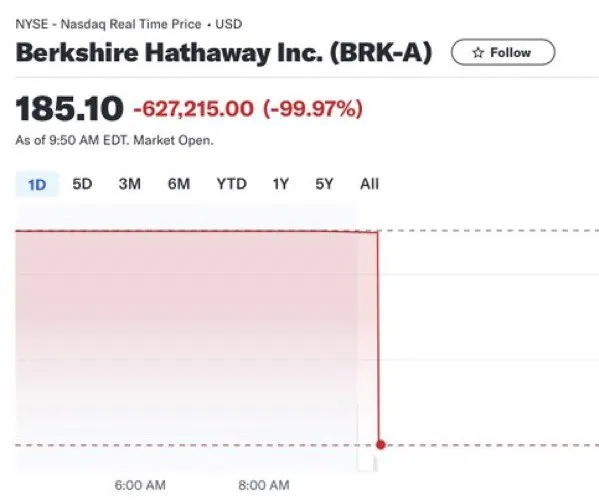
\includegraphics[width=\textwidth]{img/berkshire_crash.png}
    \end{column}
  \end{columns}
\end{frame}

\begin{frame}{Probleme durch Computerarithmetik}{Integer Overflow}
  \begin{columns}
    \begin{column}{0.6\textwidth}
      \small
      \inputminted{c}{src/zahlensysteme_ueberlauf.c}
    \end{column}
    \begin{column}{0.4\textwidth}
      Ausgabe:

      \texttt{Max int value: 2147483647} \\
      \texttt{After overflow: -2147483648}
    \end{column}
  \end{columns}
\end{frame}

\section{Überblick}

\begin{frame}{Zahlensysteme}
  \begin{itemize}
    \item Ein Zahlensystem legt die jeweiligen Regeln fest, wie Zahlen als Ziffernfolge dargestellt werden können \textrightarrow Anordnung der Ziffern festlegen
    \item Ein Zahlensystem legt fest, welcher Wert einer Ziffernfolge zugeordnet ist (A = 10, 1010 = 10 usw.) \textrightarrow Vorschrift zur Ermittlung des Zahlenwerts festlegen
    \item (Gleiche) Zahlen lassen sich in unterschiedlichen Zahlensystemen in verschiedener Form darstellen
  \end{itemize}

  \begin{block}{Unterscheidung}
    \begin{itemize}
      \item Additionssysteme
      \item Stellenwertsysteme (Positionssysteme)
      \item Hybrid-Systeme
    \end{itemize}
  \end{block}
\end{frame}

\begin{frame}{Additionssysteme}
  \begin{itemize}
    \item Jede Ziffer hat einen festen Wert
    \item Der Wert einer Ziffernfolge ergibt sich aus der Summe der Werte der einzelnen Ziffern
          \begin{exampleblock}{Unärsystem}
            Im Unärsystem wird jede Zahl durch eine wiederholte Ziffer dargestellt. Zum Beispiel wird die Zahl 3 als 111 dargestellt.
          \end{exampleblock}
          \begin{exampleblock}{Römische Zahlen}
            Die römischen Zahlen sind ein Additionssystem. Die Ziffern I, V, X, L, C, D und M haben die Werte 1, 5, 10, 50, 100, 500 und 1000.

            Besonderheit: Die Ziffernfolge wird von links nach rechts gelesen. Ist eine Ziffer kleiner als die nächste, wird sie subtrahiert.

            Beispiel: Die Zahl IX wird als 9 interpretiert, da I (1) vor X (10) steht.
          \end{exampleblock}
  \end{itemize}
\end{frame}

\begin{frame}{Stellenwertsysteme}
  \begin{itemize}
    \item Jede Ziffer hat einen festen Wert
    \item Der Wert einer Ziffernfolge ergibt sich aus der Summe der Produkte der Ziffern mit den zugehörigen Potenzen der Basis
          \begin{exampleblock}{Dezimalsystem}
            Im Dezimalsystem haben die Ziffern die Werte 0 bis 9. Die Basis ist 10.

            Beispiel: Die Zahl 1234 wird als $1 \cdot 10^3 + 2 \cdot 10^2 + 3 \cdot 10^1 + 4 \cdot 10^0 = 1234$ interpretiert.
          \end{exampleblock}
          \begin{exampleblock}{Binärsystem}
            Im Binärsystem haben die Ziffern die Werte 0 und 1. Die Basis ist 2.

            Beispiel: Die Zahl 1011 wird als $1 \cdot 2^3 + 0 \cdot 2^2 + 1 \cdot 2^1 + 1 \cdot 2^0 = 11$ interpretiert.
          \end{exampleblock}
  \end{itemize}
\end{frame}

\begin{frame}{Stellenwertsysteme}{Darstellung natürlicher Zahlen}
  In der Informatik verwenden wir in der Regel vier Zahlensysteme:
  \begin{table}
    \begin{tabular}{lrrr}
      \toprule
      System            & Basis & Ziffern                                        & Beispiel \\
      \midrule
      Binärsystem       & 2     & 0, 1                                           & 1011     \\
      Oktalsystem       & 8     & 0, 1, 2, 3, 4, 5, 6, 7                         & 1234     \\
      Dezimalsystem     & 10    & 0, 1, 2, 3, 4, 5, 6, 7, 8, 9                   & 1234     \\
      Hexadezimalsystem & 16    & 0, 1, 2, 3, 4, 5, 6, 7, 8, 9, A, B, C, D, E, F & 4D2      \\
      \bottomrule
    \end{tabular}
  \end{table}
\end{frame}

\begin{frame}{Stellenwertsysteme}{Unterscheidung (Mathematik)}
  \textbf{Welchen Wert hat 1010?}

  In der Informatik ist es wichtig, die Basis des Zahlensystems zu kennen, um den Wert einer Ziffernfolge zu bestimmen.

  \begin{block}{Konvention}
    Zur eindeutigen Darstellung von Zahlen in verschiedenen Zahlensystemen wird die Basis oft als Index hinter der Zahl geschrieben. Zum Beispiel wird die Zahl 1010 im Binärsystem als $1010_2$ und im Dezimalsystem als $1010_{10}$ dargestellt.
  \end{block}

\end{frame}

\begin{frame}{Stellenwertsysteme}{Unterscheidung}
  \textbf{Wie mache ich denn einen Index in Python?}

  Antwort: Gar nicht. Stattdessen gibt es unterschiedliche Möglichkeiten, Python zu sagen, dass eine Zahl in einem bestimmten Zahlensystem dargestellt ist.

  \begin{table}
    \begin{tabular}{ll}
      \toprule
      Zahlensystem & Darstellung in Python \\
      \midrule
      Binär        & \texttt{0b1010}       \\
      Oktal        & \texttt{0o1234}       \\
      Dezimal      & \texttt{1234}         \\
      Hexadezimal  & \texttt{0x4D2}        \\
      \bottomrule
    \end{tabular}
  \end{table}
\end{frame}

\begin{frame}{Stellenwertsysteme}{Darstellung}
  \begin{columns}
    \begin{column}{0.5\textwidth}
      \begin{itemize}
        \item natürliche Zahlen

              \( \mathbb{N} = \{1, 2, \ldots\} \)
        \item ganze Zahlen

              \( \mathbb{Z} = \{\ldots, -2, -1, 0, 1, 2, \ldots\} \)
        \item rationale Zahlen

              \( \mathbb{Q} = \left\{\frac{a}{b} \mid a, b \in \mathbb{Z}, b \neq 0\right\} \)
        \item reelle Zahlen

              \( \mathbb{R} \)
      \end{itemize}
    \end{column}
    \begin{column}{0.5\textwidth}
      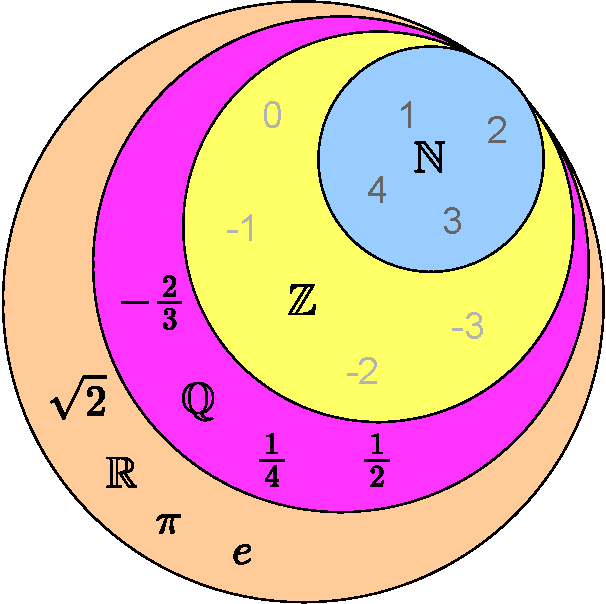
\includegraphics[width=.8\textwidth]{img/zahlensysteme_mengen.pdf}
    \end{column}
  \end{columns}

\end{frame}

\begin{frame}{Stellenwertsysteme}{Darstellung natürlicher Zahlen}
  \begin{columns}
    \begin{column}{0.5\textwidth}
      \begin{block}{Darstellung als Potenz}
        Jede natürliche Zahl \(n\) lässt sich als eine Summe von Potenzen einer beliebigen anderen natürlichen Zahl \(B \geq 2 \) darstellen in der Form
        \[
          n = \sum_{i=0}^{N-1} z_i \cdot B^i
        \]
        darstellen
        \begin{itemize}
          \item \(B\) = Basis des Zahlensystems (\(B \geq 2\))
          \item \(z_i\) = i-te Ziffer der Darstellung (\(0 \leq z_i < B\))
          \item \(N\) = Anzahl der Ziffern
        \end{itemize}
      \end{block}
    \end{column}
    \begin{column}{0.5\textwidth}
      \begin{tabularx}{\textwidth}{lrX}
        \toprule
        System            & Basis & Ziffern                                        \\
        \midrule
        Binär             & 2     & 0, 1                                           \\
        Oktalsystem       & 8     & 0, 1, 2, 3, 4, 5, 6, 7                         \\
        Dezimalsystem     & 10    & 0, 1, 2, 3, 4, 5, 6, 7, 8, 9                   \\
        Hexadezimalsystem & 16    & 0, 1, 2, 3, 4, 5, 6, 7, 8, 9, A, B, C, D, E, F \\
        \bottomrule
      \end{tabularx}
    \end{column}
  \end{columns}
\end{frame}

\begin{frame}{Stellenwertsysteme}{Darstellung natürlicher Zahlen}
  \begin{columns}
    \begin{column}{0.5\textwidth}
      \begin{block}{Darstellung als Potenz}
        Jede natürliche Zahl \(n\) lässt sich als eine Summe von Potenzen einer beliebigen anderen natürlichen Zahl \(B \geq 2 \) darstellen in der Form
        \[
          n = \sum_{i=0}^{N-1} z_i \cdot B^i
        \]
        darstellen
        \begin{itemize}
          \item \(B\) = Basis des Zahlensystems (\(B \geq 2\))
          \item \(z_i\) = i-te Ziffer der Darstellung (\(0 \leq z_i < B\))
          \item \(N\) = Anzahl der Ziffern
        \end{itemize}
      \end{block}
    \end{column}
    \begin{column}{0.5\textwidth}
      \begin{exampleblock}{Beispiel: Dezimalsystem}
        \smaller
        \begin{align*}
          2021 & = \sum_{i=0}^{3} z_i \cdot 10^i                                     \\
               & = z_0 \cdot 10^0 + z_1 \cdot 10^1 + z_2 \cdot 10^2 + z_3 \cdot 10^3 \\
               & = 1 \cdot 10^0 + 2 \cdot 10^1 + 0 \cdot 10^2 + 2 \cdot 10^3         \\
               & = 1 \cdot 1 + 2 \cdot 10 + 0 \cdot 100 + 2 \cdot 1000               \\
               & = 1 + 20 + 0 + 2000                                                 \\
               & = 2021_{10}
        \end{align*}
      \end{exampleblock}
    \end{column}
  \end{columns}
\end{frame}

\begin{frame}{Stellenwertsysteme}{Darstellung natürlicher Zahlen}
  \begin{columns}
    \begin{column}{0.5\textwidth}
      \begin{block}{Darstellung als Potenz}
        Jede natürliche Zahl \(n\) lässt sich als eine Summe von Potenzen einer beliebigen anderen natürlichen Zahl \(B \geq 2 \) darstellen in der Form
        \[
          n = \sum_{i=0}^{N-1} z_i \cdot B^i
        \]
        darstellen
        \begin{itemize}
          \item \(B\) = Basis des Zahlensystems (\(B \geq 2\))
          \item \(z_i\) = i-te Ziffer der Darstellung (\(0 \leq z_i < B\))
          \item \(N\) = Anzahl der Ziffern
        \end{itemize}
      \end{block}
    \end{column}
    \begin{column}{0.5\textwidth}
      \begin{exampleblock}{Beispiel: Binärsystem}
        \smaller
        \begin{align*}
          10110 & = \sum_{i=0}^{4} z_i \cdot 2^i                                                  \\
                & = z_0 \cdot 2^0 + z_1 \cdot 2^1 + z_2 \cdot 2^2 + z_3 \cdot 2^3 + z_4 \cdot 2^4 \\
                & = 0 \cdot 2^0 + 1 \cdot 2^1 + 1 \cdot 2^2 + 0 \cdot 2^3 + 1 \cdot 2^4           \\
                & = 0 \cdot 1 + 1 \cdot 2 + 1 \cdot 4 + 0 \cdot 8 + 1 \cdot 16                    \\
                & = 0 + 2 + 4 + 0 + 16                                                            \\
                & = 22_{10}
        \end{align*}
      \end{exampleblock}
    \end{column}
  \end{columns}
\end{frame}

\begin{frame}{Stellenwertsysteme}{Darstellung natürlicher Zahlen}
  \begin{columns}
    \begin{column}{0.5\textwidth}
      \begin{block}{Darstellung als Potenz}
        Jede natürliche Zahl \(n\) lässt sich als eine Summe von Potenzen einer beliebigen anderen natürlichen Zahl \(B \geq 2 \) darstellen in der Form
        \[
          n = \sum_{i=0}^{N-1} z_i \cdot B^i
        \]
        darstellen
        \begin{itemize}
          \item \(B\) = Basis des Zahlensystems (\(B \geq 2\))
          \item \(z_i\) = i-te Ziffer der Darstellung (\(0 \leq z_i < B\))
          \item \(N\) = Anzahl der Ziffern
        \end{itemize}
      \end{block}
    \end{column}
    \begin{column}{0.5\textwidth}
      \begin{exampleblock}{Beispiel: Hexadezimalsystem}
        \smaller
        \begin{align*}
          1C & = \sum_{i=0}^{1} z_i \cdot 16^i   \\
             & = z_0 \cdot 16^0 + z_1 \cdot 16^1 \\
             & = 12 \cdot 16^0 + 1 \cdot 16^1    \\
             & = 12 \cdot 1 + 1 \cdot 16         \\
             & = 12 + 16                         \\
             & = 28_{10}
        \end{align*}
      \end{exampleblock}
    \end{column}
  \end{columns}
\end{frame}

\begin{frame}{Stellenwertsysteme}{Darstellung von Wertebereichen}
  \begin{columns}
    \begin{column}{0.3\textwidth}
      \begin{block}{Zahlenkreis (endlich)}
        \centering
        \resizebox{\textwidth}{!}{
          \begin{tikzpicture}[rotate=90]

            \draw[thick] (0:3cm) arc (0:-360:3cm);
            \foreach \i in {0,...,3}
              {
                \draw(-\i * 20:3cm) -- (-\i * 20:3.5cm) node[above] {\i};
              }
            \foreach \i in {4,...,18}
              {
                \draw(-\i * 20:3cm) -- (-\i * 20:3.5cm) node[right] {};
              }
            \draw(1 * 20:3cm) -- (1 * 20:3.5cm) node[above] {$B^n -1$};
            \draw(2 * 20:3cm) -- (2 * 20:3.5cm) node[above] {$B^n -2$};
          \end{tikzpicture}
        }
      \end{block}
    \end{column}
    \begin{column}{0.7\textwidth}
      \begin{alertblock}{Problem}
        Während die natürlichen Zahlen unendlich sind, können wir in technischen Systemen nur mit endlichen Zahlen arbeiten.
      \end{alertblock}
      \begin{block}{Eigenschaft}
        Die Repräsentation von Zahlen in einem Computer ist immer auf eine gewisse Anzahl von Bits (Stellen im Binärsystem) beschränkt.
      \end{block}
      \begin{exampleblock}{Beispiele}
        \centering
        \begin{tabular}{cccc}
          \toprule
          \textbf{Basis} & \textbf{Stellen} & \textbf{Zahlen} & \textbf{Werte}                   \\
          \midrule
          10             & 3                & $10^3$ = 1000   & {000, 001, 002, \ldots~998, 999} \\
          2              & 3                & $2^3$ = 8       & {000, 001, 010, \ldots~110, 111} \\
          \bottomrule
        \end{tabular}
      \end{exampleblock}

    \end{column}

  \end{columns}

\end{frame}

\begin{frame}{Binärzahl und Dualzahl}
  \begin{alertblock}{Besonderheit der Deutschensprache}
    \begin{center}
      Binärzahl $\not\equiv$ Dualzahl
    \end{center}

    Die Begriffe Dual- und Binärzahl werden oft synonym verwendet. In der deutschen Sprache  sind die Begriffe jedoch voneinander abzugrenzen (im Gegensatz zur englischen Sprache \enquote{dual number} und \enquote{binary number} werden synonym verwendet).
  \end{alertblock}
  \begin{columns}[onlytextwidth]
    \begin{column}{0.48\textwidth}
      \begin{block}{Binärzahl}
        Zur Darstellung werden zwei beliebige Zeichen verwenden. (z. B. 0 und 1 oder + und -)
      \end{block}
    \end{column}
    \begin{column}{0.48\textwidth}
      \begin{block}{Dualzahl}
        Zahl in einem Stellenwertsystem zur Basis 2. (Ziffern 0 und 1).
      \end{block}
    \end{column}
  \end{columns}
  \begin{block}{Regel}
    \begin{center}
      Dualzahl $\rightarrow$ Binärzahl
    \end{center}
  \end{block}
\end{frame}

\section{Konvertierung natürlicher Zahlen}

\begin{frame}{Konvertierung natürlicher Zahlen}{Wege}
  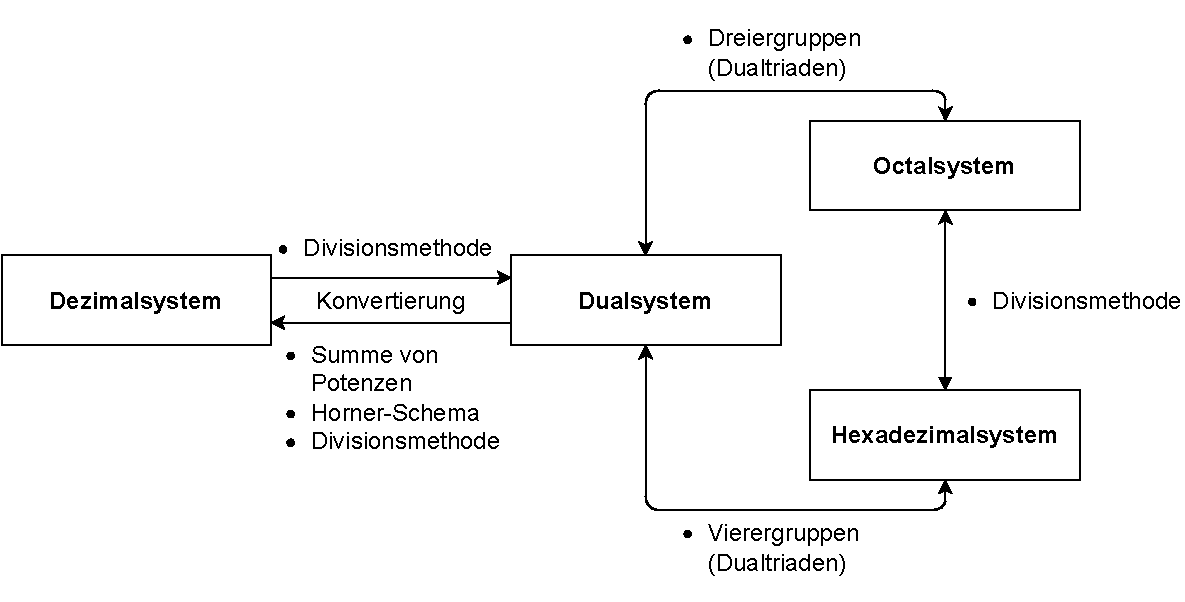
\includegraphics[width=\textwidth]{fig/zahlensysteme_umwandlung.pdf}
\end{frame}

\begin{frame}{Konvertierung natürlicher Zahlen}{Wege (Wertebeispiel)}
  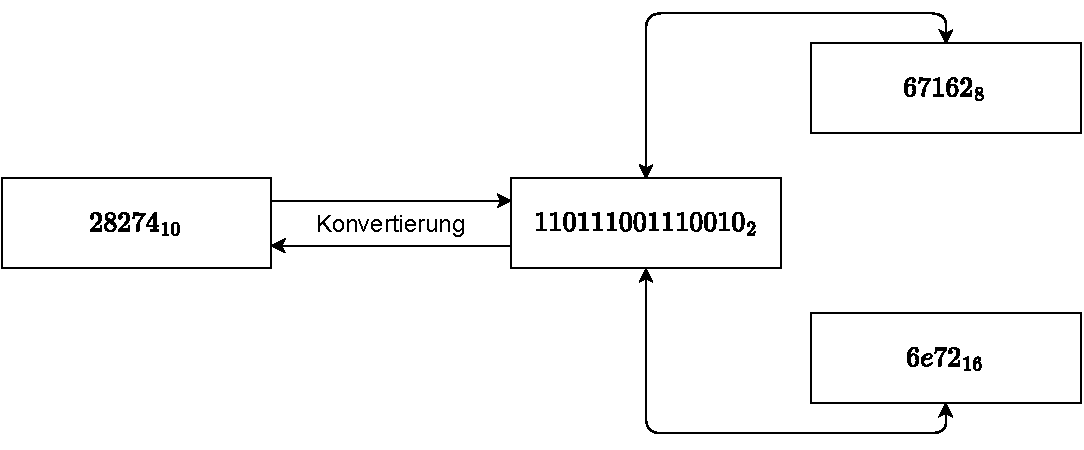
\includegraphics[width=\textwidth]{fig/zahlensysteme_umwandlung_werte.pdf}
\end{frame}

% End document
\end{document}
